\documentclass{CLGPY}

\usepackage{diagbox}

\usepackage{listings}
\usepackage{cncolours}
\lstset{
    basicstyle=\small\ttfamily,%整体格式设置
    columns=fullflexible,%设置字符列为非等宽
    breaklines=true,%自动换行
    % frameround=ttff,%边框四角弧度,t则弧
    frame=tb,%边框样式
    backgroundcolor=\color{赤金!15},%背景颜色
    framerule=1.5pt,%边框线宽度
    rulecolor=\color{墨色},%边框线颜色
    % framesep=.5em,%边距
    numbers=left,%左边显示数字
    % numbersep=0em,
    xleftmargin=2em,
    framexleftmargin=2em,
    numberstyle={\sffamily\footnotesize\color{teal}}
}

\lstdefinelanguage{latex}{
    morecomment=[l]{\%},
    commentstyle=\color{lightgray},
    morekeywords={begin,end},
    keywordstyle=\color{blue!50!black},
    morekeywords={[2]documentclass,usepackage},%导言区命令
    keywordstyle={[2]\color{red!75!black}},
    morekeywords={[3]juanqi,title,author,institute,sxrq,jjxm,zzjj,txzz,xinxi,Title,Author,Institute,keywords,enkeywords,document,abstract,enabstract,minipage,tabular,tikzpicture,multicols,includegraphics,caption,captionof,center,quad,qquad,parbox,centering,subcaption,animateinline,bibliographystyle,cite,nocite,bibliography,textbf,enumerate,itemize,toprule,bottomrule,midrule,thebibliography,bibitem,small,footnotesize,verb},%命令和环境
    keywordstyle={[3]\color{cyan!70!black}},
    morekeywords={[4]maketitle,Maketitle,figure,table},
    keywordstyle={[4]\color{朱红}},
    morekeywords={[5]CLGPY,ctexart,ctexbook,ctexrep,book,article,report,standalone,tikz,tikz-3dplot,animate,ctex,fontspec,multicol,caption,subcaption,natbib,float,booktabs,geometry,graphicx,color,xcolor,hyperref,amsmath,mathtools,siunitx,mathabx},%文类和宏包
    keywordstyle={[5]\color{竹青}},
    morekeywords={[6]part,chapter,section,subsection,subsubsection,paragraph,subparagraph},%章节
    keywordstyle={[6]\color{琥珀}},
    morekeywords={[7],newcommand,newenvironment,renewcommand,renewenvironment,def,edef,gdef,xdef}%定义类命令
    keywordstyle={[7]\color{blue!70!black}},
}
\lstnewenvironment{latexcode}
{\lstset{language=latex}}
{}
%--------------------以下命令是为了写说明文档而定义的,实际使用时可不管------------------------------%
\def\ts#1{\textcolor{red}{#1}}%提示命令
\def\bzx#1#2{$\underbracket[.5pt][1pt]{\text{#1}}_{\textcolor{red}{\text{#2}}}$}%下标注命令
\def\bzs#1#2{$\overbrace{\text{#1}}^{\textcolor{red}{\text{#2}}}$}%上标注命令
% \def\xbz#1#2{\vtop{\halign{##\crcr \hfil #1\hfil\crcr \noalign{\nointerlineskip\textcolor{red}{\hrule}\kern1pt} \hfil\small\textcolor{red}{#2}\hfil\crcr}}}%一个失败的尝试
\def\BibTeX{{%
\rm
B%
\kern-.05em%
{%
\sc
i%
\kern-.025em %
b%
}%
\kern-.08em
T%
\kern-.1667em%
\lower.7ex\hbox{E}%
\kern-.125em%
X%
}}%bibtex样式定制


\juanqi{ }{ }%卷期填写
\title[阿拉果圆盘的实现与探讨]{阿拉果圆盘的实现与探讨}
\author[黄瑞轩,校媛]{黄瑞轩,校媛}
\institute{({中国科学技术大学{\kern.5\ccwd} 计算机科学与技术学院,安徽{\kern.5\ccwd}合肥})}

\begin{document}
    \maketitle

    \begin{abstract}%中文摘要环境
        法拉第(Michael Faraday,1791—1867)于1831年发现的电磁感应现象是科学史上最重要的发现之一。而法拉第对此现象的发现与研究是与其对阿拉果圆盘实验现象的研究和解释紧密相关的。本文从阿拉果圆盘的实现出发,分析其构造、原理并探讨与其相关的一些应用。
    \end{abstract}
    \keywords{电磁感应;阿拉果圆盘;单极电动机;实验}

    \begin{multicols}{1}

        \section{阿拉果圆盘实验的历史及相关研究情况}
        \subsection{阿拉果的研究}
        1822年,阿拉果(F. J. D. Arago, 1786—1853)在测量地磁场强度时偶然发现:

\emph{·放在铜底座上的小磁针的摆动比孤立放置的小磁针摆动的幅度衰减的要快。}

\emph{·放在铜底座上的小磁针相比孤立放置的小磁针,摆动的周期无明显改变。}

他据此推测,如果静止的铜片能够影响磁针的运动,那运动的铜片也可能会对静止的磁针产生作用。

        1824年,阿拉果根据这个现象又做了一个实验。将一个圆铜盘装在轴上,使其可以自由转动,再在铜盘正上方悬下一根磁针。实验发现:

\emph{·当铜盘旋转时,磁针跟着一起旋转。}

\emph{·当磁针旋转时,铜盘也会跟着旋转。}

\emph{·在上述两种情形下,从动的那一个物体旋转稍有滞后。}

这个实验现象被称作“阿拉果圆盘效应”。
        \subsection{巴比奇和赫歇尔的研究}
1825年,巴比奇(Charles Babbage, 1791—1871)和赫歇尔(John Herschel, 1792—1871)重做了阿拉果实验并给出解释。他们认为当铜盘转动时,铜盘受到磁体的感应而显示磁性,磁体的两个磁极分别在铜盘相应的两个部分感应出了异名磁极。这种磁感应是比较特殊的感应,当铜盘和磁体静止时不发生感应,只有当磁体或铜盘存在相对运动时,感应才发生。他们将这种性质称之为Magnetic Susceptibility(磁性感受性)。

巴比奇和赫歇尔还发现了与此实验有关的“铜盘割裂效应”,当铜盘存在裂口时(铜盘在切向上不连续),不会有感应发生,但用锡将裂口焊接,感应则恢复如初;而用金属颗粒填塞裂口时,感应能力会大大降低。




        \subsection{法拉第的研究}
       1825年12月,法拉第做了一个实验,试图通过模仿阿拉果实验来产生感应电流。

        \emph{用丝线水平悬挂一根Deluc水银柱,使之可以自由转动,一个铜盘在其下旋转——没有作用。}

        \emph{一个莱顿瓶外部用导线箍住,莱顿瓶的内外壁分别充以正电和负电,当铜盘在其下旋转时,除了铜盘产生的风动效果以外,没有任何效应产生。}
       
后者是为了验证巴比奇和赫歇尔的解释。将莱顿瓶内外壁分别充上正负电荷,外壁正电以导线引出,模仿磁体的一极,内壁负电模仿磁体的另一极。法拉第认为莱顿瓶内外壁的正负电的作用类似磁铁的N极和S极,可以在转动的铜盘内同样感应出正负电,从而产生感应电流,但他尚不知感应电流属瞬时效应,因此未能观察到现象。

        \begin{figure}[H]
            \centering
            \begin{minipage}{.47\linewidth}
                \centering
                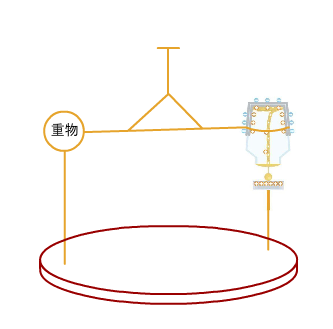
\includegraphics[width=\linewidth]{./fig/20210615085951.png}
                \caption{莱顿瓶和铜盘作用\label{fig:Laton}}
            \end{minipage}
            \quad
            \begin{minipage}{.47\linewidth}
                \centering
                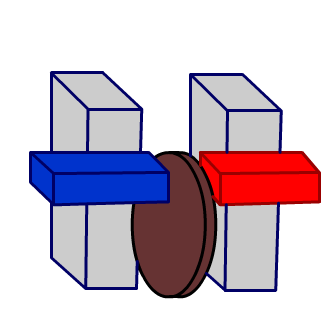
\includegraphics[width=\linewidth]{./fig/20210615090952.png}
                \caption{圆盘装置示意图\label{fig:99}}
            \end{minipage}
        \end{figure}
\newpage
        1831年10月,在发现电磁感应现象后不久,因为不满足于获得短暂的感应电流,法拉第利用圆铜盘和强磁体,设计了一套新的实验装置,产生出稳恒的感应电流。

        (\emph{首先})\emph{为了强化磁极作用,两个小磁体放置在两个大磁体磁极的前端,小磁体与磁极横向交叉,并且小磁体的较宽的一面紧贴磁极,使两个小磁体的两端靠的足够近;为了防止震动引起的滑动,用绳子把它们紧紧地绑在一起。}

        \emph{圆盘边缘插放在两个强化磁极之间,边缘与汞混合。与圆盘同样厚度的铜条末端弯成凹槽,同样与汞混合,以便能与圆盘的边缘良好接触。两根这样的铜条用丝线绑在一个纸板上,以便它们能同时和圆盘边缘比较相近的两个点同时接触,这些接触器通过导线与电流计连接。当圆盘以一定速度转动时,产生稳恒的电流。}

        

        起初,法拉第认为在圆盘中产生了涡旋电流,所以他将接触器放在磁极间圆盘的两侧,结果几乎测不到电流。多次更换位置后,他发现当两个接触器触点分别处于边缘和轴心时,电流最大。根据圆盘转向的不同以及磁极的不同,感应电流从轴心流向边缘或从边缘流向轴心。

        11月,法拉第利用一个实验说明了巴比奇和赫歇尔发现的铜盘割裂效果,间接上也说明了阿拉果实验效应完全是铜盘内感应电流的结果:

        \emph{两片铜板,每片的直线边缘都与汞混合,放在一起使其穿过磁极,电流计效应强烈;再把一张纸放在边缘之间,电流计没有可察觉到的效应。}

        \begin{center}
            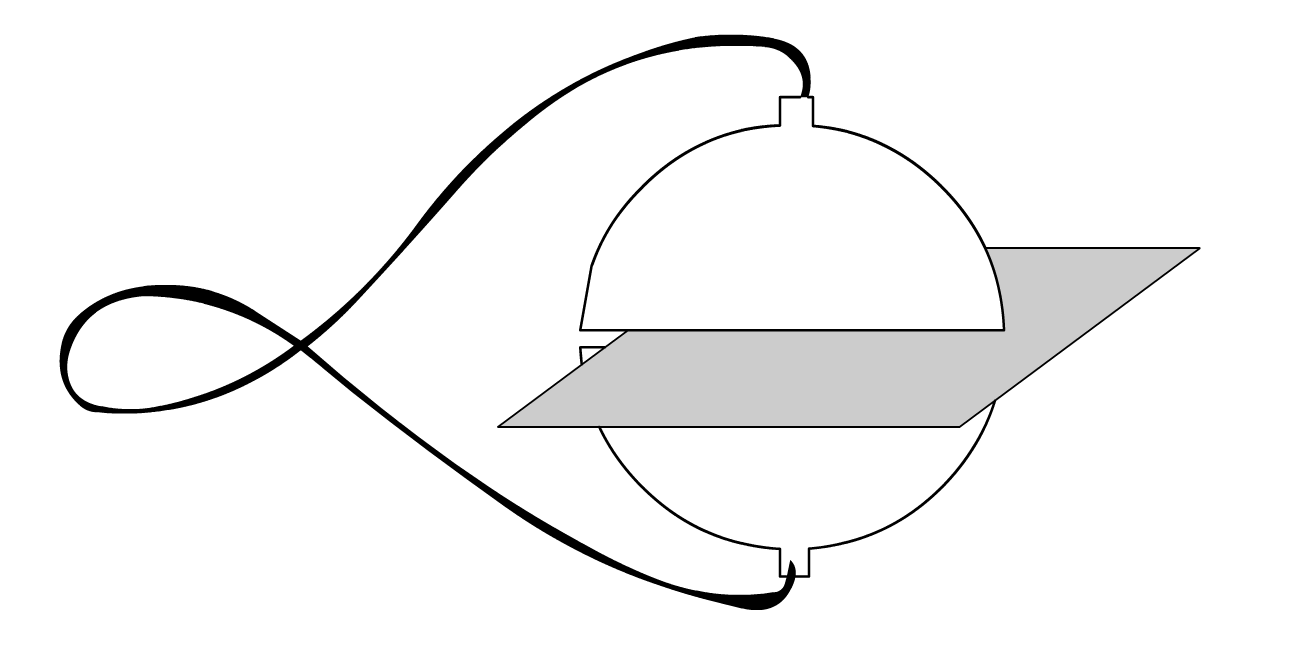
\includegraphics[scale=.14]{./fig/20210615103816.png}
            \captionof{figure}{接合铜板示意图\label{fig:99}}
        \end{center}
   
        这是因为,当“每片的直线边缘都与汞混合”,两块铜板成为一个导体。穿过磁极时,产生的感应电流通过这完整的回路在电流计上显示效应;而当“仅把一张纸放在边缘之间”,就产生了铜盘存在裂口的效果。此时两块铜板不再是一个完整的导体,因此电流计就不会产生效应。

        12月,法拉第又通过一个实验,再次说明了当阿拉果圆盘转动时,是铜盘和磁体的相对运动产生了感应电流:


        \emph{仅利用地磁做阿拉果实验。不用磁体,圆盘水平放置并旋转,电流计磁针的效应虽轻微但很明显,并且可以通过铜盘复原并多次旋转等动作,使磁针效应增加。当圆盘如标示的方向转动时,磁针的方向向东。这里没用铁,如果电流计内的导线和导体都用粗导线,可能有更强的效应。}

\emph{因此阿拉果的铜盘是个新的发电机。}
        \begin{center}
            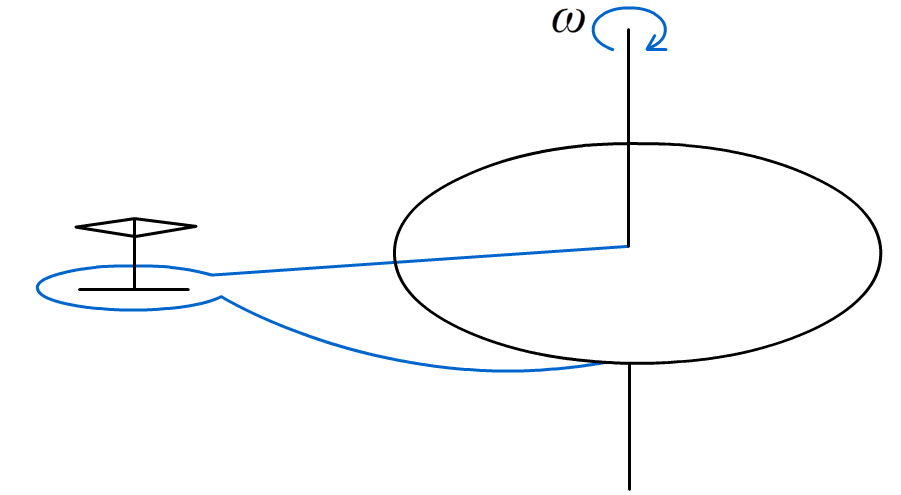
\includegraphics[scale=.18]{./fig/20210615111946.png}
            \captionof{figure}{圆盘地磁感应示意图\label{fig:99}}
        \end{center}

之后,法拉第结合自己之前做的实验,反驳了巴比奇和赫歇尔的理论,用阿拉果效应为自己的电磁感应理论充当了有力的论据。




     \section{阿拉果圆盘效应的电磁学原理}
     \subsection{磁场的模拟}
首先我们要知道外磁场的情况。在这一实验中,外界磁场是小磁针所产生的磁场,可以近似认为是磁偶极子产生的磁场,而圆形载流细导线回路可以看作是一个磁偶极子。如图所示,导线线径忽略,导线上电流以线电流$I=I_0$来作近似。

        \begin{center}
            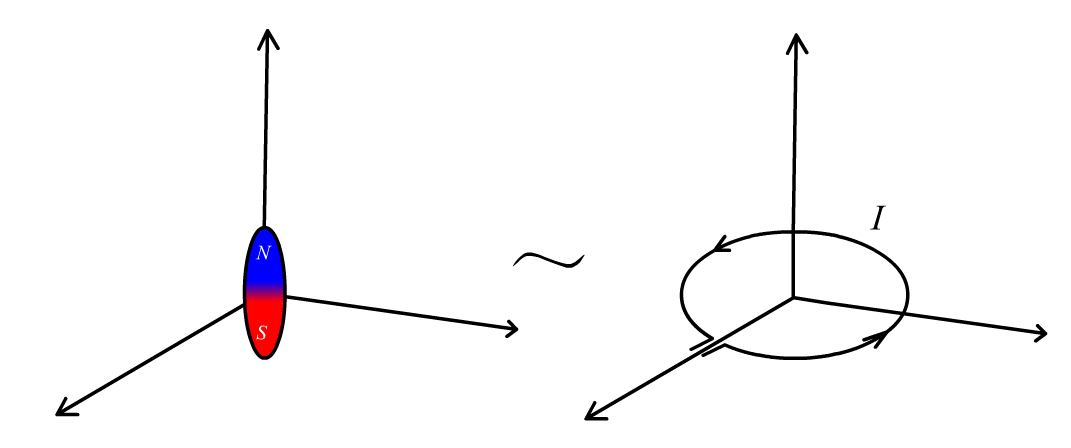
\includegraphics[scale=.2]{./fig/20210615122211.png}
            \captionof{figure}{等效模型示意图\label{fig:99}}
        \end{center}

该磁偶极子的偶极矩
\begin{equation}
\bm{\mu}=I_0\bm{S}=I_0S\bm{e_z}
\end{equation}

这个磁偶极子产生的磁矢势设为$\bm{A}$,则
\begin{equation}
\bm{A}(\bm{r})=\frac{\mu_0I_0}{4\pi}\int_L\frac{1}{\|\bm{r-r'}\|}\text{d}\bm{l'}
\end{equation}

令$\displaystyle f(r)=\frac{1}{r}$,则
\begin{equation}
f(\|\bm{r-r'}\|)=f(\bm{r})-\bm{r'}·\nabla f(\bm{r})+\cdots
\end{equation}

又因为
\begin{equation}
\int_{L} \text{d} \boldsymbol{l}^{\prime}=0
\end{equation}

则
\begin{equation}
\boldsymbol{A}(\boldsymbol{r})=-\frac{\mu_{0} I_{0}}{4 \pi} \int_{L} \boldsymbol{r}^{\prime} \cdot \nabla f(\boldsymbol{r}) \text{d} \boldsymbol{l}^{\prime}
\end{equation}

坐标化表示
\begin{equation}
\boldsymbol{r}^{\prime}=R \boldsymbol{e}_{\boldsymbol{r}^{\prime}}=R\left(\boldsymbol{i} \cos \varphi^{\prime}+\boldsymbol{j} \sin \varphi^{\prime}\right)
\end{equation}
\begin{equation}
\begin{aligned}
\text{d} \boldsymbol{l}^{\prime}&=\text{d} \boldsymbol{r}^{\prime}=R \boldsymbol{e}_{\varphi} \text{d} \varphi^{\prime}\\&=a\left(-\boldsymbol{i} \sin \varphi^{\prime}+\boldsymbol{j} \cos \varphi^{\prime}\right) \text{d} \varphi^{\prime}
\end{aligned}
\end{equation}
\begin{equation}
\nabla f(\bm{r})=-\frac{1}{r^{2}} \boldsymbol{e}_{\boldsymbol{r}}
\end{equation}

于是
\begin{equation}
\begin{aligned}
-\boldsymbol{r}^{\prime} \cdot \nabla f(\boldsymbol{r})&=R \boldsymbol{e}_{\boldsymbol{r}}^{\prime} \cdot \frac{1}{r^{2}} \boldsymbol{e}_{\boldsymbol{r}}\\
&=\frac{\sin \theta \cos \left(\varphi-\varphi^{\prime}\right) R}{r^{2}}
\end{aligned}
\end{equation}

所以磁矢势
\begin{equation}
\begin{aligned}
\boldsymbol{A}(\boldsymbol{r})&=\frac{\mu_{0} I_{0} R^{2}}{4 r^{2}} \sin \theta(\bm{i} \sin \varphi-\bm{j} \cos \varphi)\\&=\frac{\mu I_0 S}{4 \pi r^{2}}\left(\bm{e_z} \times \bm{e_r}\right)\\&=\frac{1}{4 \pi {r}^{3}} \bm{\mu\times r}
\end{aligned}
\end{equation}

所以要求的磁感应强度
\begin{equation}
\begin{aligned}
\boldsymbol{B}&=\nabla \times \boldsymbol{A}=\frac{1}{4 \pi r^{3}}[\boldsymbol{\mu}(\nabla \cdot \boldsymbol{r})-\boldsymbol{r}(\nabla \cdot \boldsymbol{\mu})]\\
&=\frac{\mu_0\mu(\bm{e_\theta}\sin\theta+2\bm{e_r}\cos\theta)}{4\pi r^3}
\end{aligned}
\end{equation}

在上式中,磁偶极矩是沿$z$轴方向的,利用计算机模拟可以得到这个磁场的分布情况如图所示。
        \begin{center}
            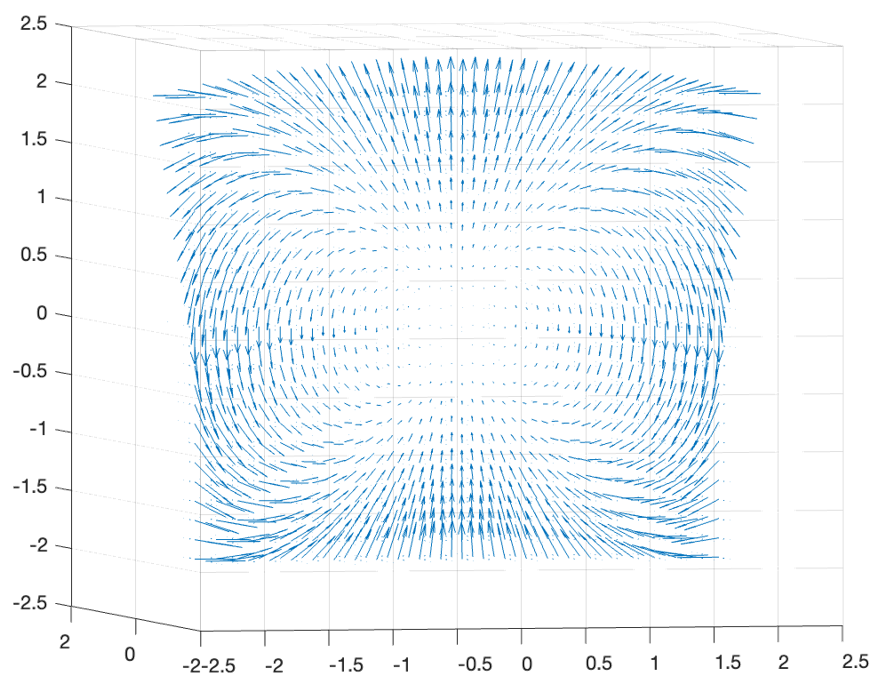
\includegraphics[scale=.2]{./fig/20210615123048.png}
            \captionof{figure}{散点图:磁场的三维分布示意图\label{fig:99}}
        \end{center}
        \begin{center}
            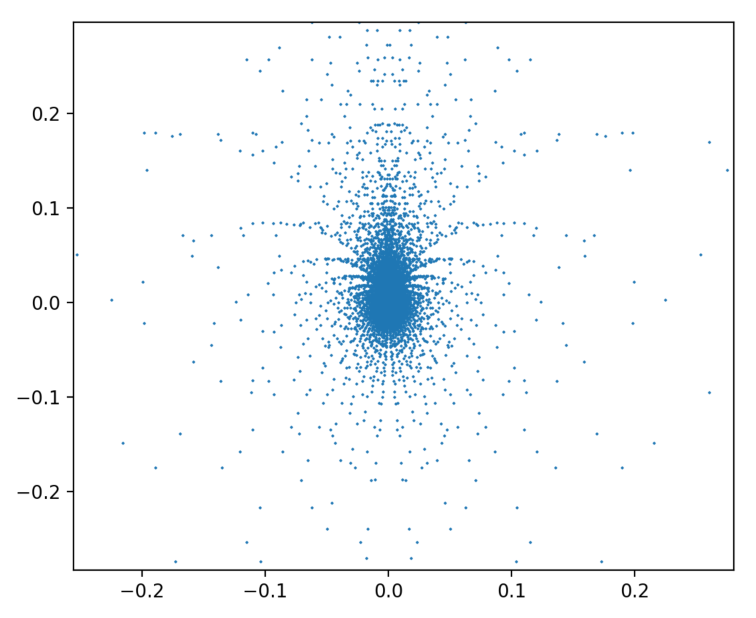
\includegraphics[scale=.2]{./fig/20210618230811.png}
            \captionof{figure}{磁场在$xOz$平面的投影\label{fig:99}}
        \end{center}

        \begin{center}
            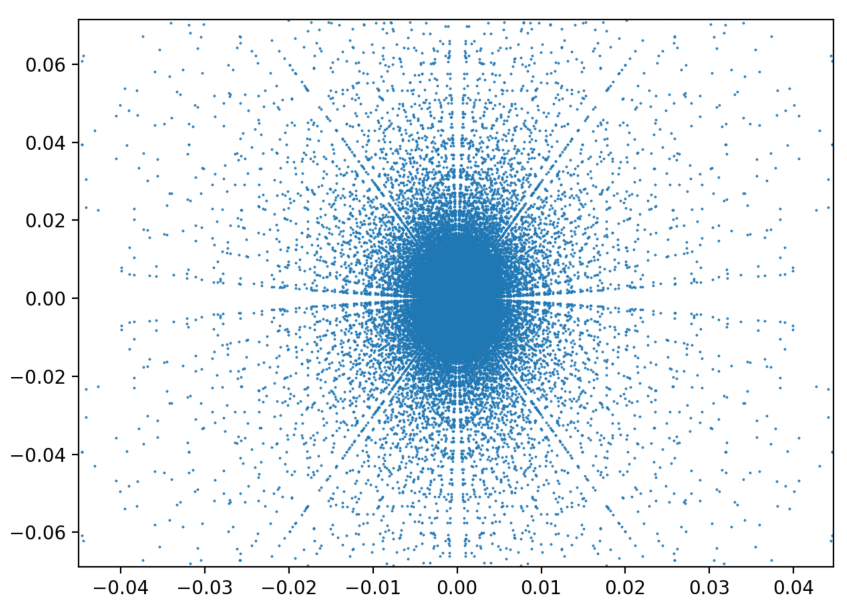
\includegraphics[scale=.2]{./fig/20210618231224.png}
            \captionof{figure}{磁场在$xOy$平面的投影\label{fig:99}}
        \end{center}

        \begin{center}
            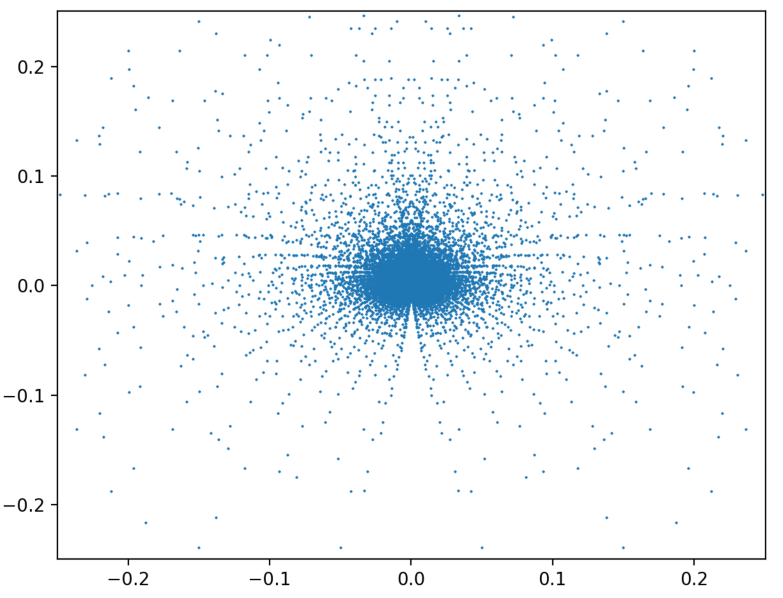
\includegraphics[scale=.2]{./fig/20210618231304.png}
            \captionof{figure}{磁场在$yOz$平面的投影\label{fig:99}}
        \end{center}

\subsection{感应电流的产生}
法拉第电磁感应定律建立在闭合导体回路之上,但是所研究的圆盘并不是闭合导体回路。笔者首先想到的是利用微元的视角,将铜圆盘分割成无数个铜圆环,研究它们产生的涡旋电流。

由于小磁针的磁场是轴对称分布,穿过圆盘的磁通量$\Phi$保持不变,因此有
\begin{equation}
\varepsilon=-\frac{\mathrm{d} \Phi}{\mathrm{d} t}=0
\end{equation}

没有感应电动势出现,而
\begin{equation}
\varepsilon=\oint \boldsymbol{E} \cdot \mathrm{d} \boldsymbol{l}
\end{equation}

这说明没有涡电流出现,与实验结果不符合。于是笔者转换思路,将圆盘看作是无数根铜棒组成的,每根铜棒上都有感应电动势产生。一根与磁铁夹角为$\alpha$的铜棒上产生的感应电动势为
\begin{equation}
\Delta \varepsilon_{\alpha}=\int_{0}^{R}\left[\left(\boldsymbol{\omega}_{t} \times \bm{r^{\prime}}\right) \times \boldsymbol{B}(r, \alpha)\right] \cdot \mathrm{d} \boldsymbol{r'}
\end{equation}


可见一根铜棒上有且仅有磁感线穿进(穿出),因此感应电流也是一侧流入一侧流出的。加之我们认为圆盘的变速过程是准静态的,即在每个研究阶段,有
\begin{equation}
\omega_t\equiv \omega_0
\end{equation}

故对于一根铜棒,有
\begin{equation}
|\Delta\varepsilon_\alpha|\neq0
\end{equation}

这说明确有沿着径向流动的电流。这些径向的电流产生的磁场在水平方向上的分量都是同向的,因此对小磁针产生一个转动力矩,所以小磁针发生了旋转。

但是根据巴比奇和赫歇尔发现的铜盘割裂效果,笔者推测,圆盘的真实结构应当是上面两种情况的叠加。铜圆环固然不参与感应电流的形成,但是参与导体回路的形成,在这个模型中也是至关重要的。
        \begin{center}
            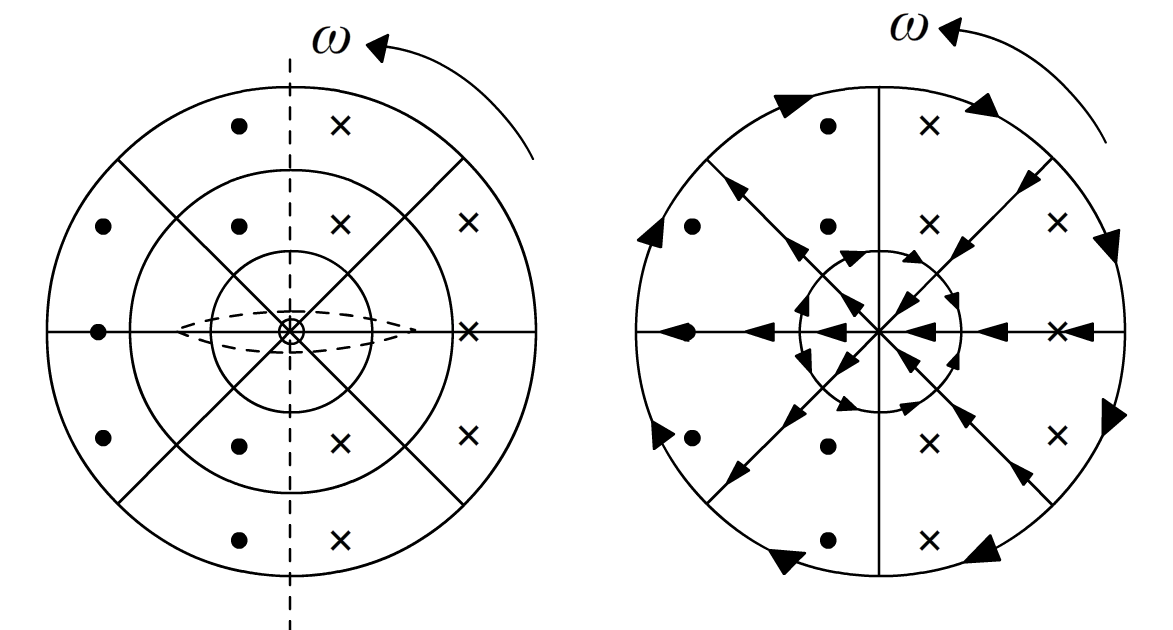
\includegraphics[scale=.16]{./fig/20210614153906.png}
            \captionof{figure}{构建的模型示意图\label{fig:model_img}}
        \end{center}

下面我们来定量计算感应电动势的大小,计算过程中用到的物理量见下图。
        \begin{center}
            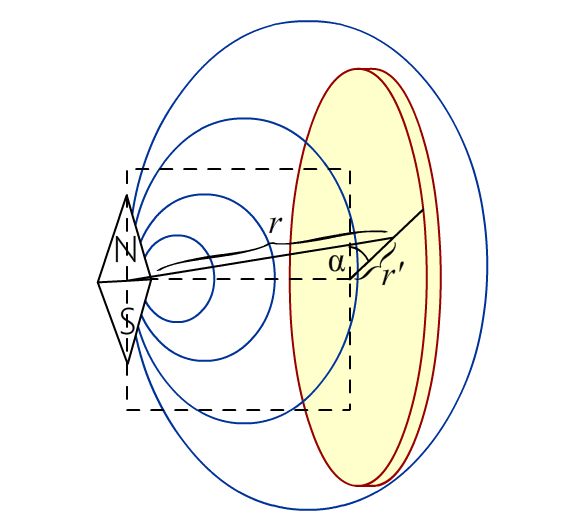
\includegraphics[scale=.28]{./fig/20210614152326.png}
            \captionof{figure}{积分示意图\label{fig:integral_img}}
        \end{center}
\begin{equation}
\begin{aligned}
\Delta \varepsilon_{\alpha}&=\int_{0}^{R}\left[\left(\boldsymbol{\omega}_{t} \times \bm{r^{\prime}}\right) \times \boldsymbol{B}(r, \alpha)\right] \cdot \mathrm{d} \boldsymbol{r'}\\
&=\int_0^R\frac{\mu_o\mu\omega r'}{4\pi(r'^2+h^2)^{5/2}}r'\cos^2\alpha(h^2-r'^2\cos2\alpha)\text{d}r'\\
&=\frac{\mu_0\mu\omega\cos^2\alpha}{4\pi}\left[\frac{3R^3+2(3h^2R+4R^3)\cos2\alpha}{6(h^2+R^2)^{3/2}}\right.\\&\text{ }\left.-\cos2\alpha\sinh^{-1}\left(\frac{R}{h}\right)\right]
\end{aligned}
\end{equation}

利用计算机对上面结果进行模拟,分别得到圆盘上某一棒上电势随$r'$的分布图、圆盘上棒的电动势随$\alpha$角变化的图。
        \begin{center}
            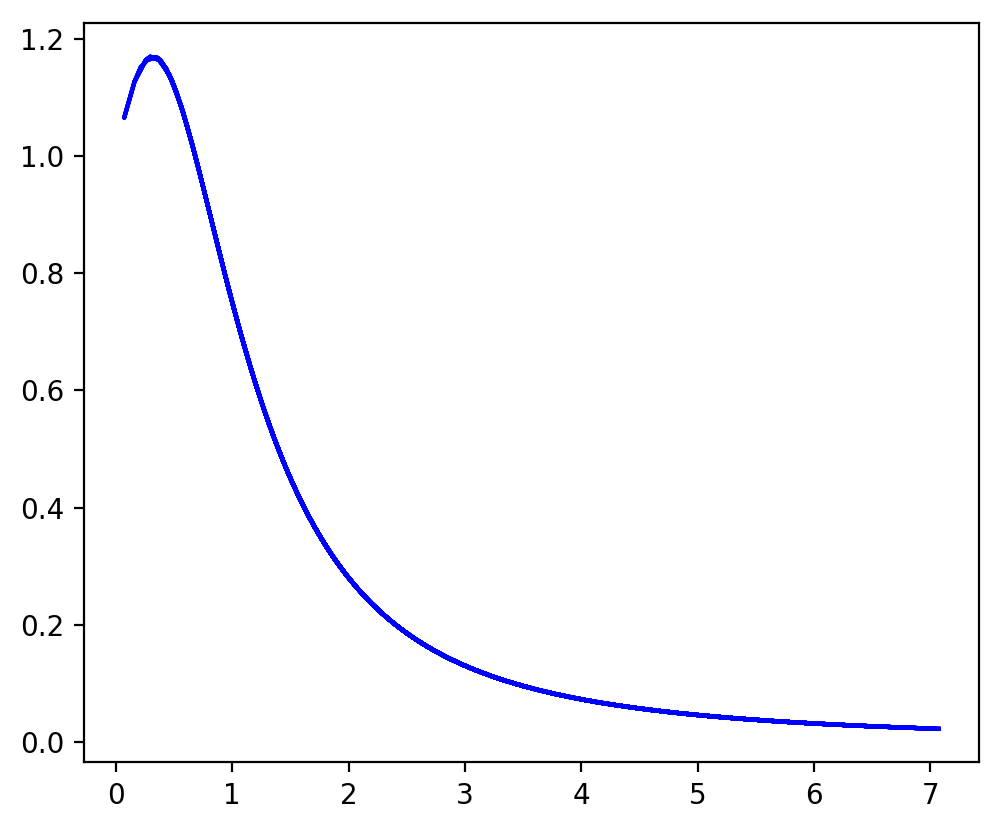
\includegraphics[scale=.2]{./fig/20210616200434.png}
            \captionof{figure}{圆盘上某一棒上电势随$r'$的分布图\label{fig:model_img}}
        \end{center}

        \begin{center}
            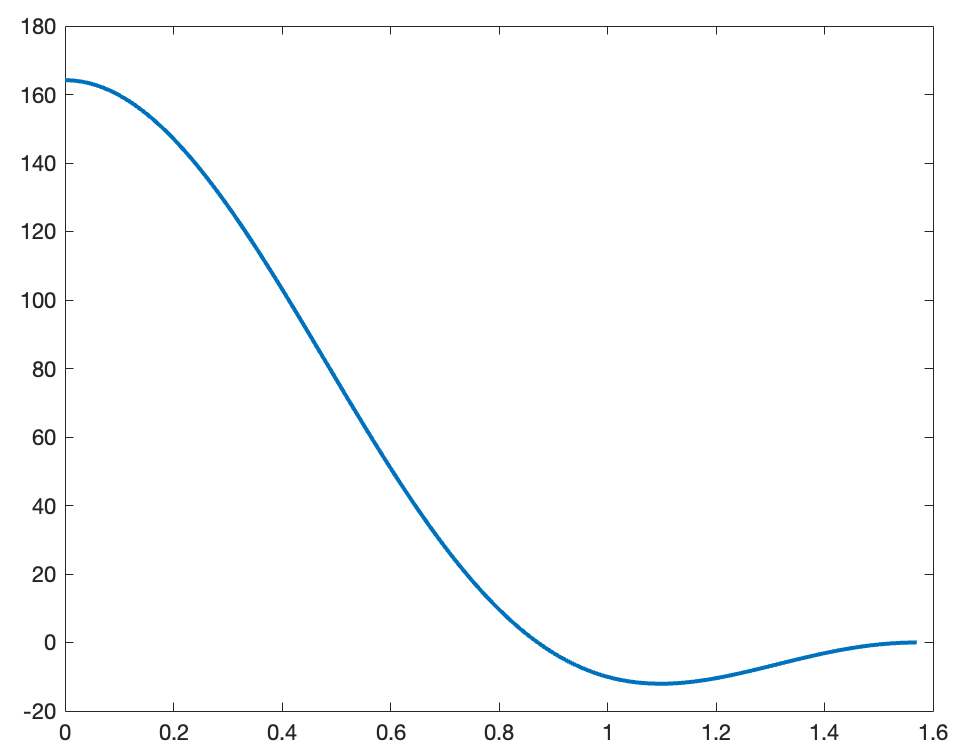
\includegraphics[scale=.21]{./fig/20210618231743.png}
            \captionof{figure}{圆盘上棒的电动势随$\alpha$角变化的图\label{fig:model_img}}
        \end{center}

注意到这样一个积分结果是$\alpha$的偶函数,这恰好证明了小磁针两侧圆盘区域的对称性。当$\alpha=0$时,感应电动势最大,对应恰好与小磁针重合的那一根铜棒;当$\alpha=90$°时,感应电动势为0,对应电流的分界线。因此可以看到,小磁针的方向与电流分界线方向是垂直的,这体现了滞后效应。

\subsection{力矩的产生}
将电动势近似看成均匀分布,简化模型为无限长导线,因此一段铜棒所产生的磁场磁感应强度
\begin{equation}
B=\frac{\mu_{0} \Delta \varepsilon_{\alpha}}{2 \pi h R_{e}}
\end{equation}

其中$R_e$是材料的电阻,由磁荷的观点,我们可以得到转动力矩
\begin{equation}
\Delta\boldsymbol{M}=\boldsymbol{H} q_{\mathrm{m}} \times \boldsymbol{r}_{\mathrm{mag}}=\frac{\mu_{0} \mu \Delta \varepsilon_{\alpha} r_{\mathrm{mag}}}{2 \pi h R_{e}} \boldsymbol{e}_{\boldsymbol{\theta}}
\end{equation}

这仅是正下方一根铜棒产生的效应,若要考虑到其他铜棒共同的效应,则应考虑一个复杂的积分。但是该积分结果形式与$\Delta\bm{M}$相同,故以$X$代替积分因子,总的力矩形式上记为
\begin{equation}
\boldsymbol{M}=\frac{\mu_{0} \mu X\Delta \varepsilon_{\alpha} r_{\mathrm{mag}}}{2 \pi h R_{e}} \boldsymbol{e}_{\boldsymbol{\theta}}
\end{equation}

由前面对感应电动势的计算,我们知道当小磁针性质、位置不变时,感应电动势仅与圆盘角速度$\omega$和所处位置$\alpha$有关,因此如果考虑一侧的电动势总和,也要涉及到一个复杂的角度积分,但是形式也不改变,故以$Y$代替积分因子,即$\varepsilon=Y\omega$,则我们可以写出这个力矩最终的表达式
\begin{equation}
\bm{M}=Z\omega \bm{e_\theta}
\end{equation}

其中$Z$是常系数。于是我们就得到了运动方程
\begin{equation}
\frac{\text{d}\omega^*}{\text{d}t}=\frac{Z}{J}\omega
\end{equation}

这里设$\omega^*$是小磁针的角速度,$J$是小磁针的转动惯量。考虑到之后的运动,我们用相对运动的观点,即可以得到适用于全程的运动方程
\begin{equation}
\frac{\text{d}\omega^*}{\text{d}t}=\frac{Z}{J}(\omega-\omega^*)
\end{equation}

这个方程表明,小磁针角速度$\omega^*$的变化始终落后于圆盘角速度$\omega$的变化(在准静态过程下),说明电磁感应理论能够正确地说明小磁针的滞后效应。

\section{阿拉果圆盘试做}
\subsection{第一次实验}
笔者准备了一个半径为3厘米的紫铜圆盘,中间打一个直径2.5毫米的孔,利用热熔胶将其固定在一个12V、9900转/分的小型马达上,用可变电源驱动;正上方用柔软的细线悬挂一个磁力摆,使其静止。调整可变电源的输出电压值,观察磁力摆的运动情况。

实验观察到如下现象:

\emph{·当电源打开时,小型马达在很短时间内就加速到匀速状态。}

\emph{·没有观察到圆盘旋转产生明显的风动。}

\emph{·磁力摆开始摆动,做类简谐运动。}

\emph{·外加电压越大,圆盘转速越快,磁力摆振幅越大。}

\emph{·断开电源,圆盘逐渐停止,磁力摆振幅开始衰减并最终回到原来的平衡位置。}


笔者使用了4V~10V的电源进行测试,用手机拍摄运动并找到振幅最大的点。实验记录如下:
        \begin{figure}[H]
            \centering
            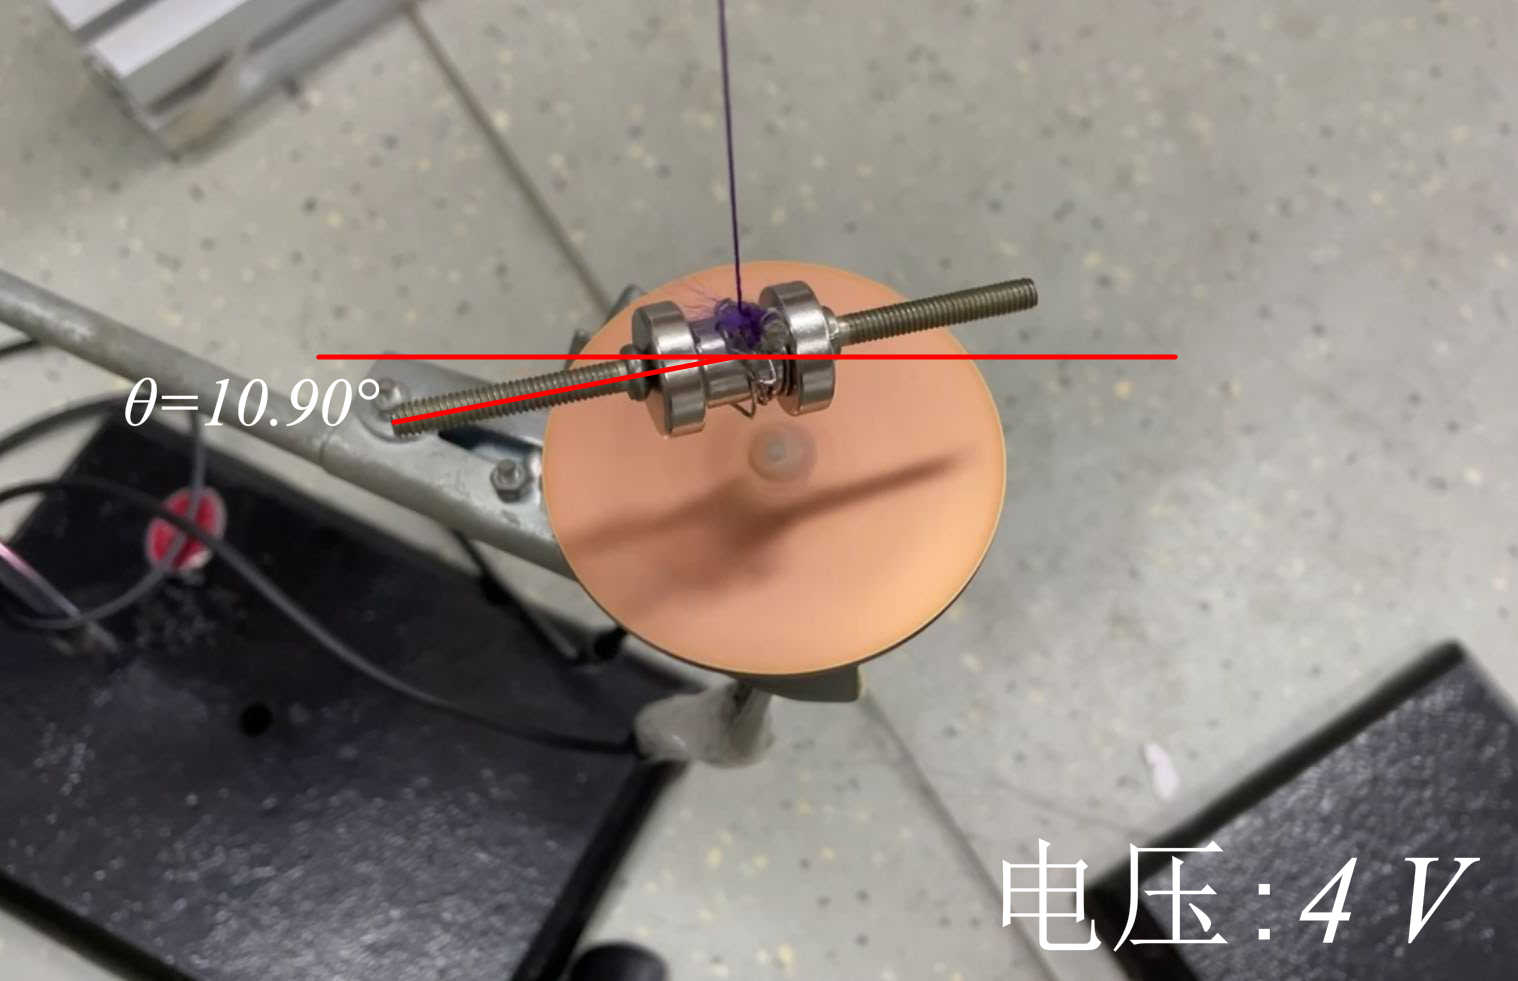
\includegraphics[width=.72\linewidth]{./fig/img1.png}\\[4pt]
            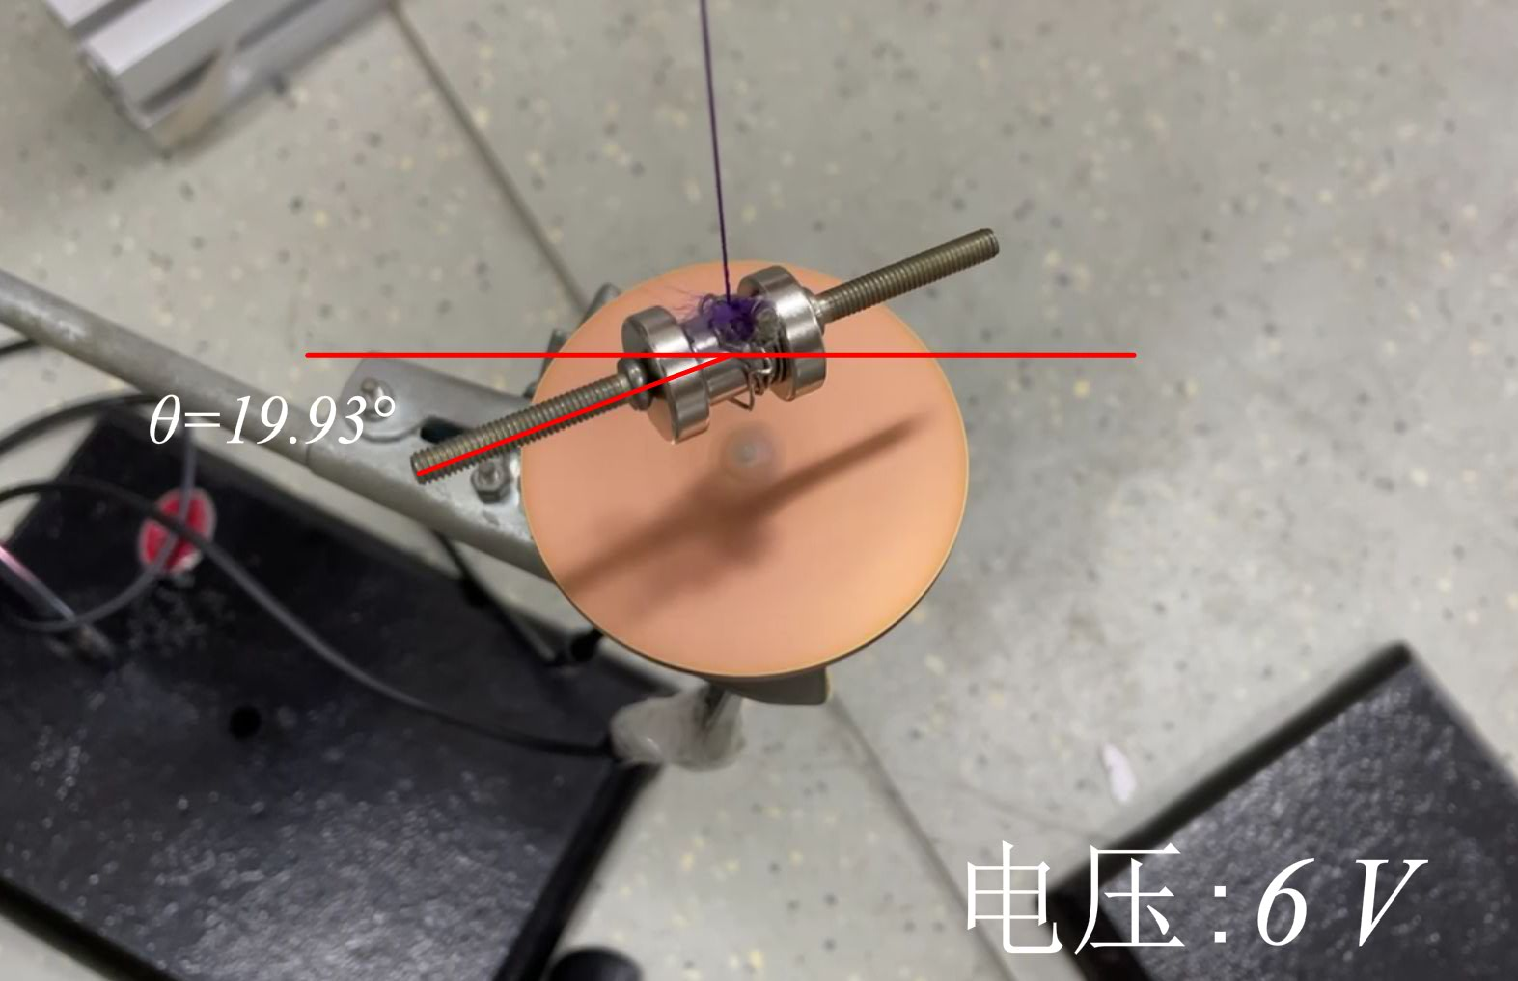
\includegraphics[width=.72\linewidth]{./fig/img2.png}\\[4pt]
            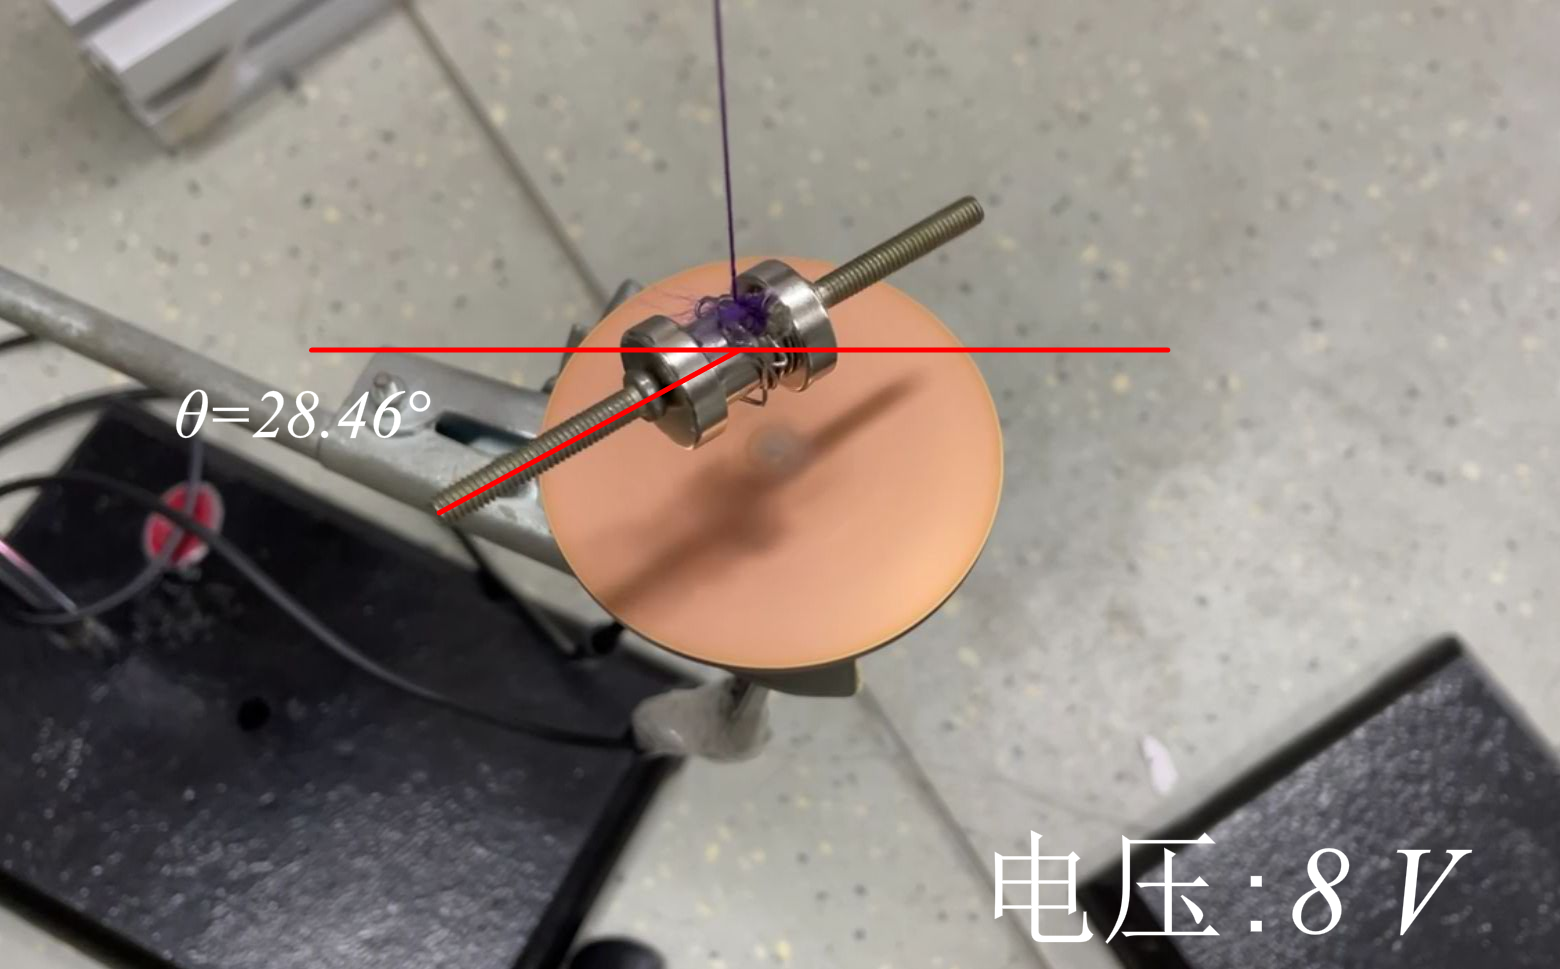
\includegraphics[width=.72\linewidth]{./fig/img3.png}\\[4pt]
            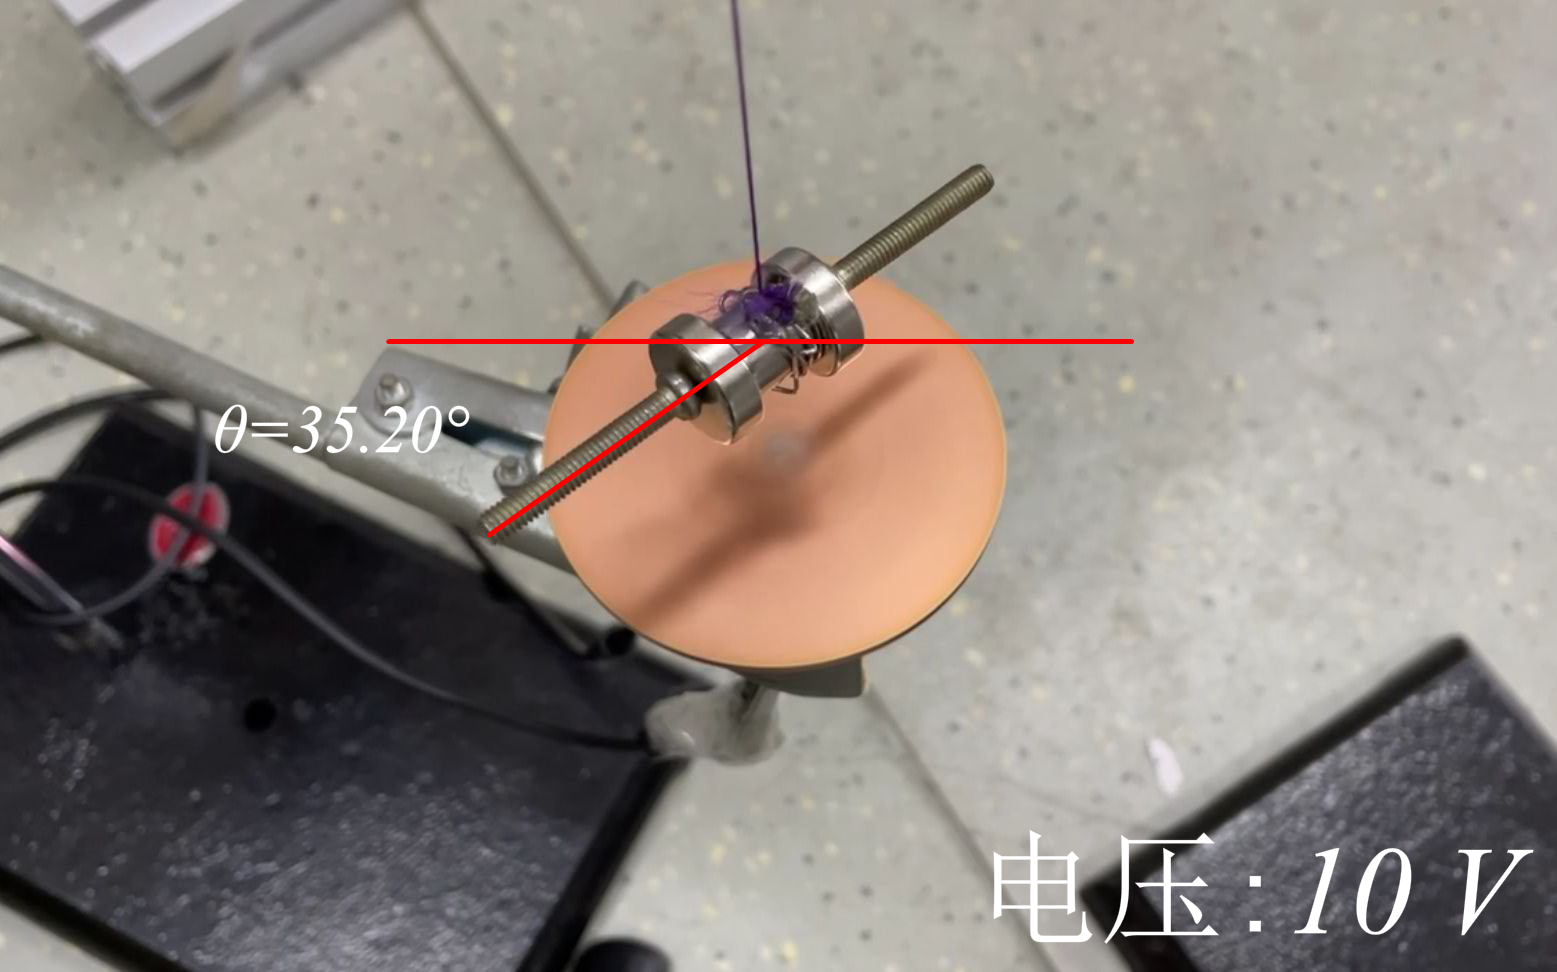
\includegraphics[width=.72\linewidth]{./fig/img4.png}\\
            \caption{不同电压下的振幅最大值记录\label{fig:dtgy}}
        \end{figure}

        \begin{center}
            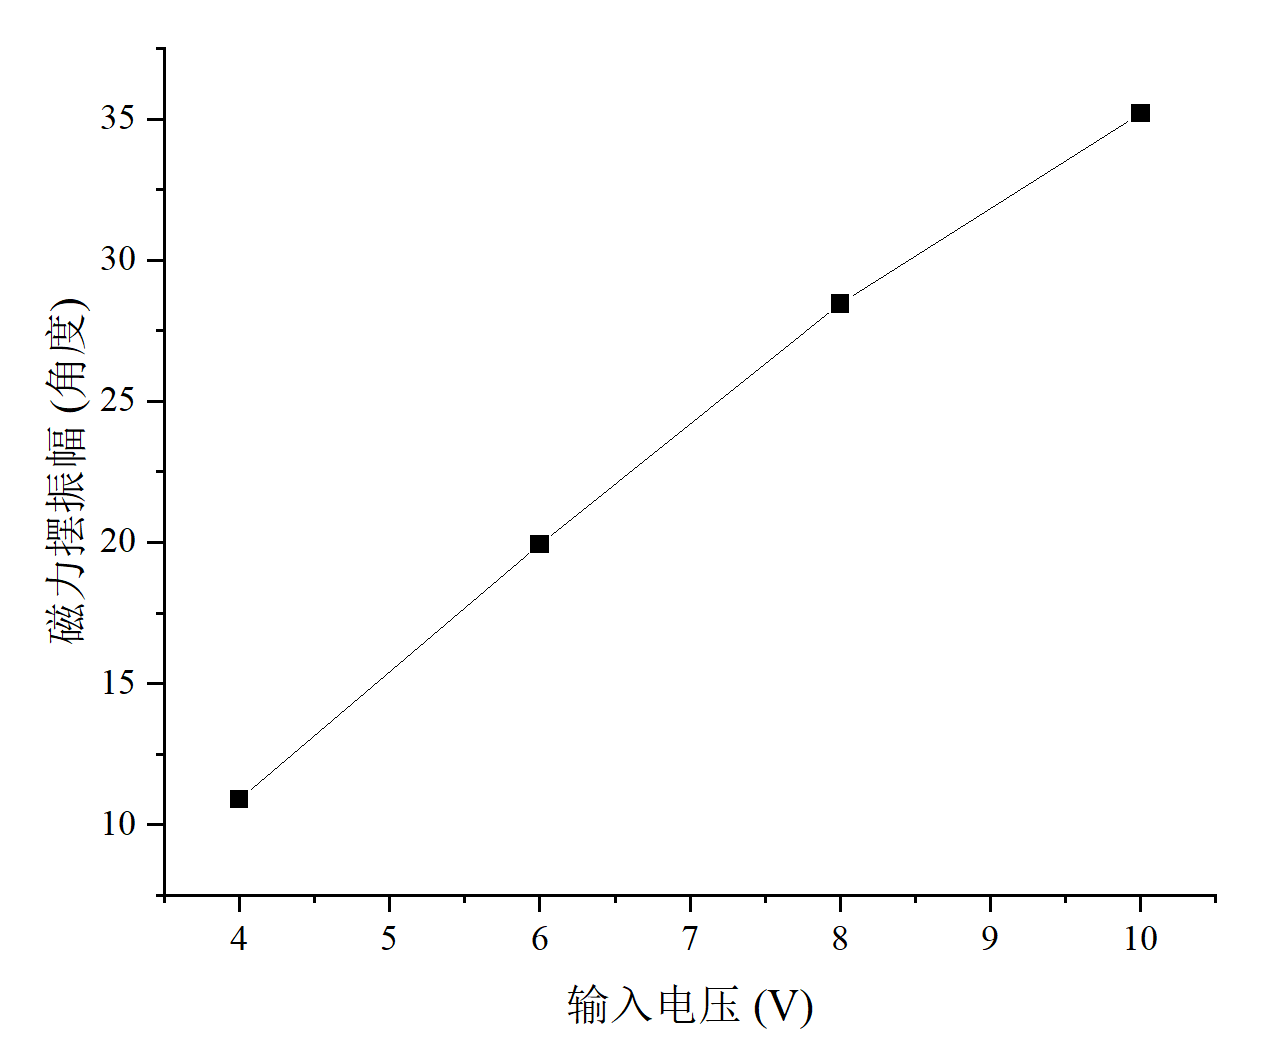
\includegraphics[scale=.18]{./fig/20210616205713.png}
            \captionof{figure}{振幅-电压散点图\label{fig:model_img}}
        \end{center}

实验中未能观察到磁力摆做电磁学模型中所述的“从动”效果,而是做一定振幅的简谐运动。进一步观察,在未放置圆盘装置前,磁力摆的指向为南北方向(地磁场方向);在放置圆盘后,磁力摆指向变为东西方向。这说明磁力摆受到了环境磁场的干扰,这个干扰强于阿拉果圆盘产生的磁场,因此磁力摆以在这个磁场中的运动为主。经过高斯计测量证明,这个干扰磁场为电动马达中永磁体产生的磁场。

经了解,笔者所用的电动马达构造如下图所示。
        \begin{figure}[H]
            \centering
            \begin{minipage}{.47\linewidth}
                \centering
                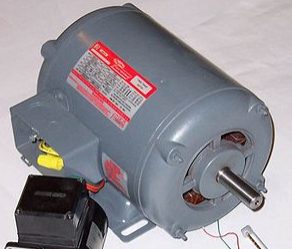
\includegraphics[width=\linewidth]{./fig/20210617221233.png}
                \caption{电动马达外形\label{fig:Laton}}
            \end{minipage}
            \quad
            \begin{minipage}{.47\linewidth}
                \centering
                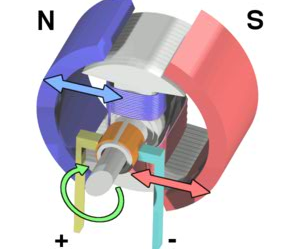
\includegraphics[width=\linewidth]{./fig/20210617221330.png}
                \caption{电动马达内部结构\label{fig:99}}
            \end{minipage}
        \end{figure}

右图所示的结构产生的磁场,可以近似看成是一个较强的匀强磁场。它穿过磁力摆,因此磁力摆离开平衡位置开始做简谐运动。
\subsection{第二次实验}
为了尽量减少电动机永磁体所带来的干扰,笔者使用一根长度约为12cm的用尽的中性笔芯作为传动装置,用热熔胶粘牢。这样可以使圆盘和磁力摆尽量远离电动机,减少后者产生磁场的干扰。为了避免离心作用使笔芯左右摆动,将笔芯穿过一个开孔略大于笔芯直径的瓦楞纸片,并用铁架台固定这一瓦楞纸片。其他步骤、配置同第一次实验。

实验观察到如下现象:

\emph{·当电源打开时,小型马达在很短时间内就加速到匀速状态。}

\emph{·没有观察到圆盘旋转产生明显的风动。}

\emph{·磁力摆很快开始做加速转动,且转动速度小于圆盘转速。}

\emph{·外加电压越大,圆盘转速越快,磁力摆的转速也越快。}

\emph{·断开电源,圆盘逐渐停止,磁力摆由于细绳被扭紧而向反方向做转动,最终停止。}

        \begin{center}
            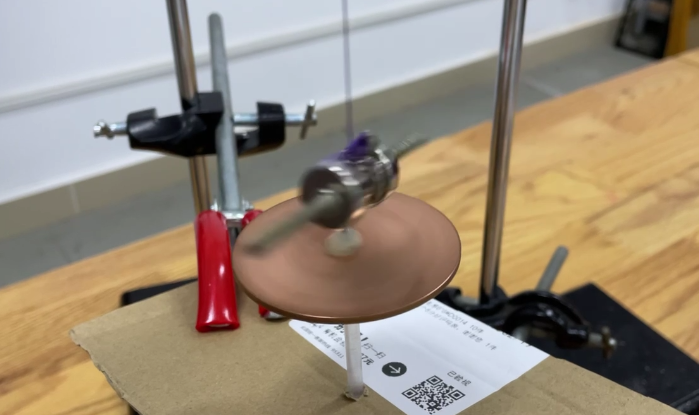
\includegraphics[scale=.3]{./fig/20210617225410.png}\\[4pt]
            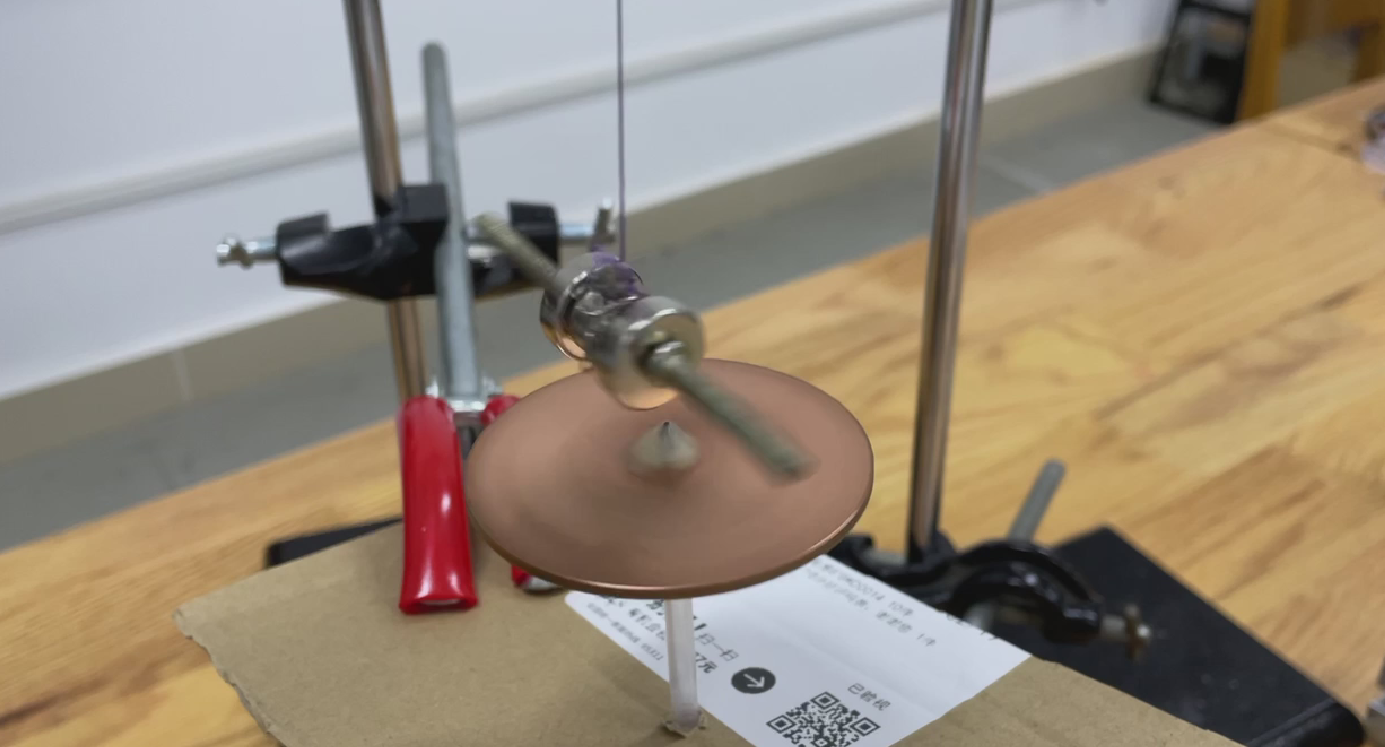
\includegraphics[scale=.152]{./fig/20210619000939.png}
            \captionof{figure}{第二次实验情况\label{fig:model_img}}
        \end{center}

笔者为实验全程录制了视频,至此,笔者成功完成了阿拉果圆盘实验的实际操作。值得指出的是,由于在磁力摆旋转过程中细线难免会偏离轴线方向,磁力摆在细线处于轴线位置时的运动是不稳定平衡,会导致接下来的转动不可控制。但是在这一现象出现之前,已经成功地观察到了阿拉果效应,如果想要再进一步改进,可以将细线换成带有可转动枢纽的细棒等。

\section{单极电动机能否用来制作阿拉果圆盘?}
\subsection{单极电动机简介}
阿拉果圆盘的搭建中用到了电动马达,其本质是一种电动机。日常生产中所用到的电动机通常是利用通电线圈产生旋转磁场,这个磁场作用于转子形成磁电动力旋转扭矩。而单极电机是指其电枢部分始终处于单极性磁场中的电机。它不需要换向器,电枢部分也不需要进行绝缘处理,但转速自然也比不上电动马达。现在我们利用单极电机来探讨在这样的转速下能否实现阿拉果圆盘现象。

笔者尝试搭建的单极电机结构如下面左图所示。这是一种结构简单、效果显著的搭建方法。将电池的一极与白色钕铁硼磁铁相吸合,利用一个矩形线框进行电流承载。这个矩形线框一端凹陷,用于接触电池的一极;另一端与磁铁两端分别接触,将电流汇入电池的另一极。

白色钕铁硼磁铁是一种可以导电的磁铁。这种磁铁可以看成一种较扁的条形磁铁,一圆面为N极,另一圆面为S极。这种磁铁产生的磁感应强度比较大,产生磁感应强度的范围也适合单极电机的尺寸,适合用来制作单极电机。
        \begin{center}
            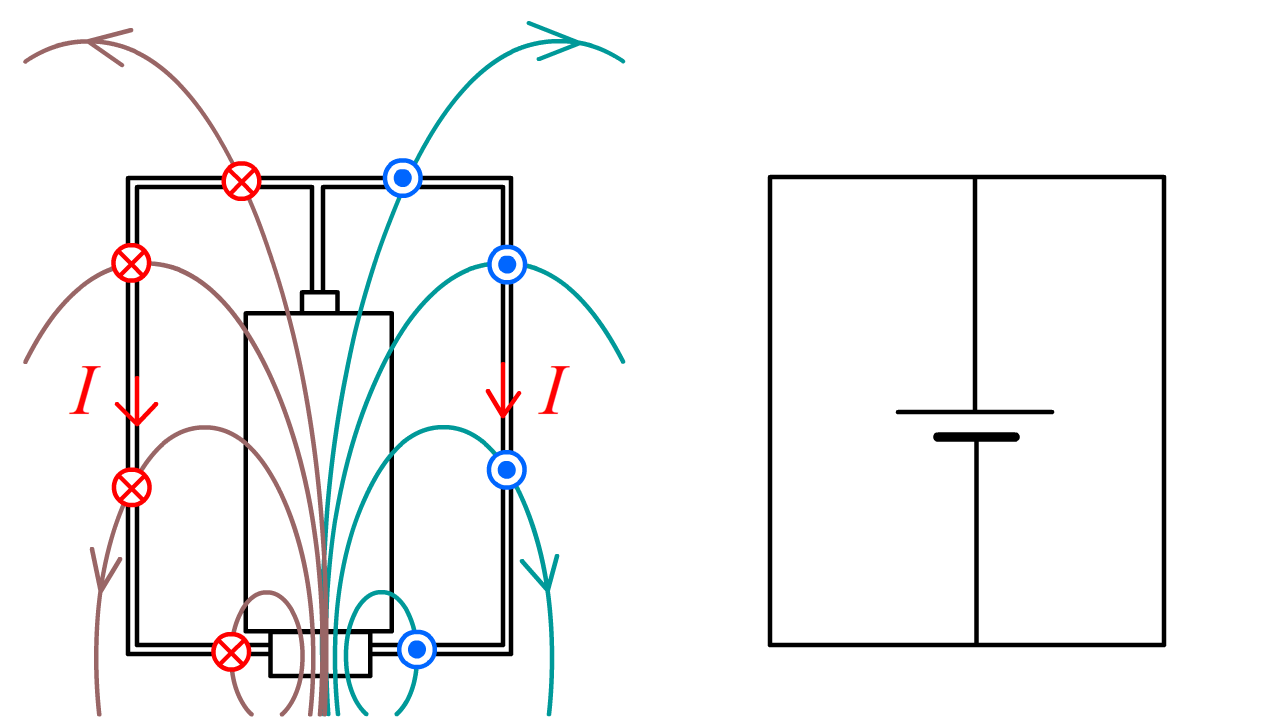
\includegraphics[scale=.15]{./fig/20210614191454.png}
            \captionof{figure}{单极电动机的构造和电路图(导线电阻未画出)\label{fig:single_mower}}
        \end{center}
\subsection{单极电动机的电磁学、动力学建模}
单极电机的结构可以抽象为上面右图所示的电路。在理想的对称情况下,两侧支路将通过相等的电流,这个电流设为$I$,外界磁场(设为$\bm{B}(\bm{r})$)是非均匀的,在矢径为$\bm{r}_0$处产生的磁场为$\bm{B}(\bm{r}_0)$,这个磁场将对该处电流元产生一个安培力,其大小为
\begin{equation}
\text{d}\bm{F}(\bm{r}_0)=I\text{d}\bm{l}\times\bm{B}(\bm{r}_0)
\end{equation}
由于两侧电流方向相同,而磁力线对称分布,由于叉乘运算具有反对称性,这个磁场在两侧产生的安培力大小相等,方向相反,不妨设其表征力为$F_A$。这个两个安培力对线圈产生同一方向的转动力矩$M=FR$,因此可以驱动线框旋转。


在现实情况下,由于存在摩擦力矩以及空气阻力力矩$M_{f(\omega)}$,这个力矩与转速相关,当$2M$接近于$M_{f(\omega)}$时,根据转动定律
\begin{equation}
J\beta=2M-M_{f(\omega)}
\end{equation}
可知,线圈的转速将趋于稳定。这个过程会因为产生焦耳热而消耗电池能量,线圈转速会逐步减弱,但在稳定后一个较短的时间内仍可认为线圈做匀速圆周运动。


由于用于搭建单极电机的材料除磁铁外都不具有磁性,实验所用的电池,除了两端电极之外不含金属导体,因此对原磁场产生的影响可以忽略。

所用电池参数显示,正常短路电流约在6A~12A,根据安培环路定理,这个电流在距离为$r$处产生的磁场为
\begin{equation}
B=\frac{\mu_{0} I}{2 \pi r}
\end{equation}

这个磁感应强度在$10^{-3}$m(毫米)量级内将衰减至$10^{-3}$T量级。实验前用精密高斯计测得磁铁在电机所处空间范围内所产生的磁感应强度大约是$10^{-1}$~$10^{-2}$T量级,因此电流产生的磁场对原磁场的分布影响在进行建模时也做忽略处理。

首先,我们还是需要对磁场建模。不妨把磁铁看成磁偶极子。磁偶极子是十分靠近的一对等量异号磁荷,磁荷量为$q_m$,距离为$l$,磁偶极矩大小为$p_m=q_ml$,方向由负磁荷指向正磁荷。这里我们用磁荷的观点,由电偶极子的分析结果,可类推出磁偶极子的磁感应强度表达式为
\begin{equation}
\boldsymbol{B}=\mu_{0} \boldsymbol{H}=-\frac{\mu_{0} \boldsymbol{\mu}}{4 \pi r^{3}}+\frac{3 \mu_{0} \boldsymbol{\mu} \cdot \boldsymbol{r}}{4 \pi r^{5}} \boldsymbol{r}
\end{equation}

用计算机模拟可以得出这个磁场分布图如下所示。
        \begin{center}
            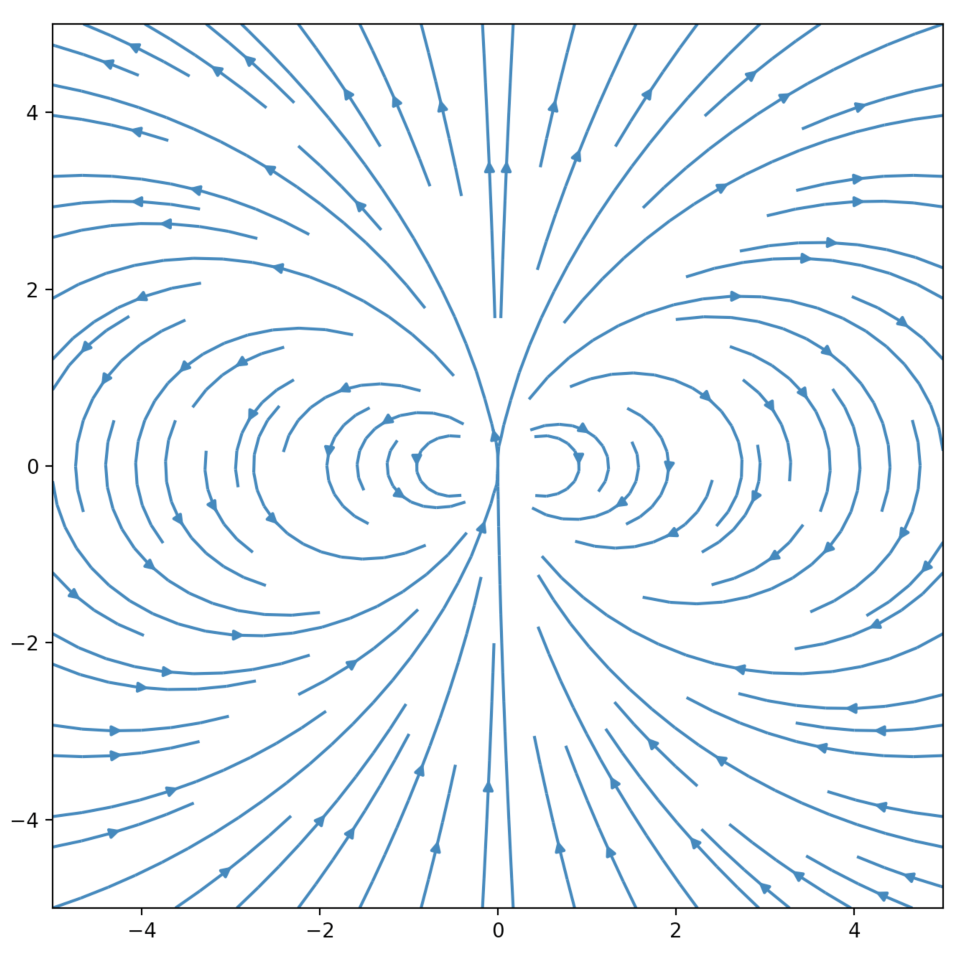
\includegraphics[scale=.2]{./fig/20210615122737.png}
            \captionof{figure}{基于Python实现的磁偶极子磁场分布图(正视图)}
        \end{center}


假设线圈半径为$R$,高度为$H$,其中的电流为$I$,则在柱坐标中研究,一侧线框受到的力矩为
\begin{equation}
\frac{1}{2}M=M_1+M_2+M_3
\end{equation}

其中
\begin{equation}
\begin{aligned}
M_{1} &=\int_{0}^{R} B(r, \theta, 0) I r \mathrm{d} r
\end{aligned}
\end{equation}
\begin{equation}
\begin{aligned}
M_{2} &=\int_{0}^{H} B(a, \theta, h) I a \mathrm{d} h 
\end{aligned}
\end{equation}
\begin{equation}
\begin{aligned}
M_{3} &=\int_{0}^{R} B(r, \theta, H) I r \mathrm{d} r
\end{aligned}
\end{equation}

合力矩为$M$,由
\begin{equation}
J\beta=2M-M_{f(\omega)}
\end{equation}
给出转动加速度。

由于在实验过程中没有竖直方向的安培力存在,由于
\begin{equation}
f=\mu N
\end{equation}
知$N$应当是常数,因此可以认为
\begin{equation}
\frac{\partial M_{f}}{\partial \omega}=0
\end{equation}
即摩擦力矩近似为常量,因此圆盘将做加速运动。受电磁感应等效应的影响,空间中的$B$、导线中的$I$要发生变化,当$\beta=0$时,开始做匀速转动。

        \begin{center}
            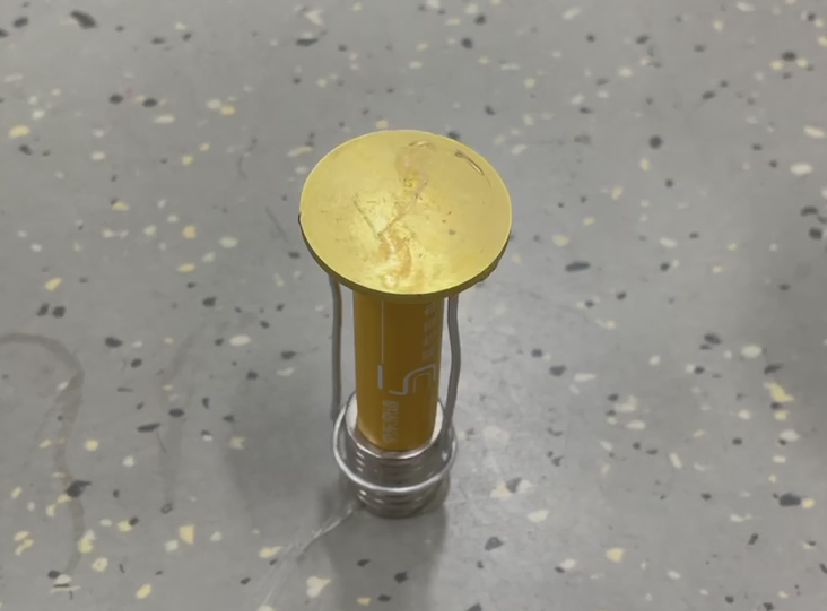
\includegraphics[scale=.15]{./fig/20210616212532.png}
            \captionof{figure}{搭建的单极电机(黄铜片、铝线)}
        \end{center}
\subsection{实际实验}
实际实验中,笔者利用锡线、铝线和铜线进行制作,最后发现使用铝线是转速最快的、最稳定的(锡线容易氧化损毁,铜线转速慢)。用热熔胶将铜圆盘固定在电机顶端,上部悬下一个磁力摆,再将高斯计置于圆盘和磁力摆之间,调零后接通电路,观察高斯计示数。

实验观察到如下现象:

\emph{·高斯计示数不变。}

\emph{·经测量,单极电动机负荷铜圆盘时的转速最大为70转/分。}


\subsection{结论}
测量出来的单极电动机转速远小于电动马达的转速,产生的磁场几乎无法测出。由于使用的电池电压比较低、电池容量也比较小,利用单极电动机驱动阿拉果圆盘的思路暂时失败了。

由于时间紧张,笔者根据该实验现象推测,如果将铜盘换成一定厚度的铜箔,并加大电池的容量,并将磁力摆换成小磁针,可能会有现象出现。这是因为铜盘太重,严重影响了单极电机的转速。

\section{展望}
\subsection{利用相对运动使阿拉果圆盘效果显著化}
阿拉果在最初的实验中描述道,放在铜底座上的小磁针的摆动,比孤立放置的磁针摆动的幅度衰减的要快。因此推测静止的圆盘对动态的小磁针产生了作用。如果用相对运动的观点来看,以小磁针为参考系,也就是动态的圆盘对静态的小磁针产生作用。因此我们可以让圆盘不动,用一个条形磁铁来加强磁场,使这个条形磁铁旋转,观察圆盘的效应和条形磁铁的角速度变化。

为了获得较大而稳定的角速度,可以使用有弹性的粗绳,这种绳子在拧紧后为了恢复原来的状态会带动条形磁铁旋转。这种旋转运动转速较大,而且比较稳定,适合本实验的研究。
\subsection{利用阿拉果圆盘制作电磁感应演示仪}
根据前面的实验,利用阿拉果圆盘可以制作电磁感应演示仪。用塑料盒将马达、铜盘和传动装置封装,灵敏电流计和铜片用电刷连接。

实验时,电源开启,此时小磁针与旋转的紫铜圆盘相对运动,圆盘内形成径向电流,可以观察到灵敏电流计发生偏转,从而演示电磁感应现象。

灵敏电流计的接脚通过槽来限定轨迹,还可以用此装置验证当导体相对磁场运动时,产生的究竟是径向电流还是涡电流。实验装置示意图如图所示。

        \begin{center}
            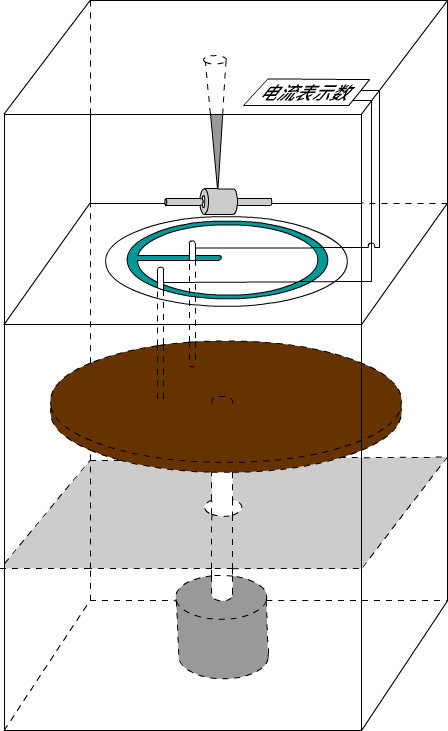
\includegraphics[scale=.3]{./fig/111.png}
            \captionof{figure}{装置示意图}
        \end{center}

\subsection{利用不同的铜丝网模型验证建模}
本文在建模时曾推测,阿拉果圆盘可以看作一种铜丝网模型。若要验证,可以尝试制作不同的铜丝网模型,用这些模型来替代阿拉果圆盘,用灵敏电流计检测各现象是否出现,以此来验证建模的正确性。

        \begin{center}
            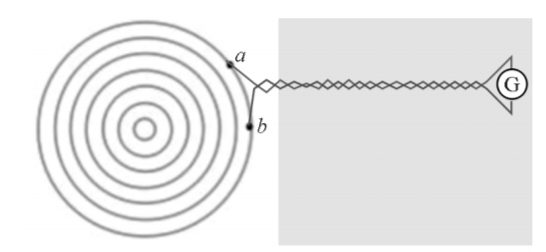
\includegraphics[scale=.3]{./fig/20210619133325.png}\\[3pt]
            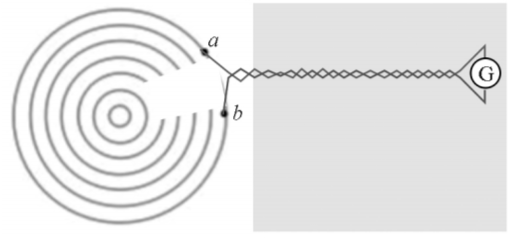
\includegraphics[scale=.3]{./fig/20210619133334.png}\\[3pt]
            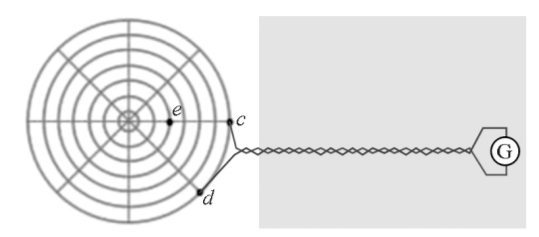
\includegraphics[scale=.3]{./fig/20210619133344.png}\\[3pt]
            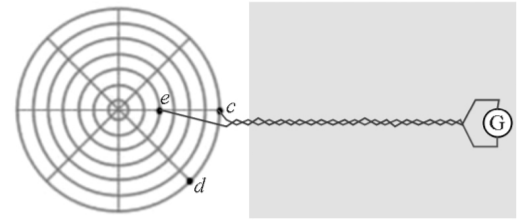
\includegraphics[scale=.3]{./fig/20210619133353.png}
            \captionof{figure}{可行的一种对照方案}
        \end{center}
\section{结语}
从理论分析到实际操作,笔者成功地复原了阿拉果圆盘效应。阿拉果圆盘启发了法拉第制作成电动机,具有丰富的内涵和实践意义。这一效应作为电磁感应的一种表现,可以在非接触的情况下使物体旋转,可以用来制造电磁感应演示模型或者类似磁力搅拌器之类的装置。

同时,阿拉果圆盘作为一种结构简单、现象明显的电磁感应效应,用来制作电磁感应定律演示仪是非常简便有效的,可以为初学电磁感应定律的学生们增添学习电磁学的兴趣与乐趣。

\section{致谢}
作为一个实验类的题材,笔者在理论到实践操作的转换之间遇到了许许多多的问题。在这里要感谢物理实验中心的韦先涛、王中平和朱玲老师对本课题所需要用到的实验器材和实验场地的支持;感谢工程实验中心的叶回春老师为实验器材加工方面的支持;感谢笔者的电磁学任课教师卢荣德老师和助教陈越对实验的指导。

法拉第在一生的探索中遭遇了多次失败。在他当年的日记里,“毫无反应”“不行”等词语,记录着艰苦的探索历程。几十年的经历使他在晚年感叹道:“就是最有成就的科学家,得以实现的建议、猜想和初步判断,也不到十分之一。”虽然笔者经过一些理论分析和试做,已经初步建立了模型。但是由于时间紧迫,仍没有制造出比较适宜的演示装置。怀揣着对物理先贤的崇敬以及对物理实验的热情,笔者仍会在不远的将来继续完善这一课题。

\begin{thebibliography}{99}  
\bibitem{ref1}FARADAY M.Thomas Martin Ed. Faraday's Diary[M]. Vol. 1. London: G. Bell and Sons, Ltd, 1932.
\bibitem{ref2}王洛印. 法拉第对阿拉果铜盘实验现象的研究和解释[J]. 哈尔滨工业大学学报, 2010, 12(4): 8-12.  
\bibitem{ref3}Jesse M. Kinder, Philip Nelson. Python物理建模初学者指南[M]. 河北: 人民邮电出版社, 2017.
\bibitem{ref4}郭鑫. 单极电动机的电磁分析与试验研究[D]. 西南交通大学硕士学位论文, 2015, 5. 
\bibitem{ref5}黄绍书. 阿拉果铜盘实验的实验研究与分析[J]. 物理通报, 2016(7): 97-100.
\end{thebibliography}

\end{multicols}
\Title{The Making and Discussion of Arago's Disc}
\Author{HUANG Ruixuan, XIAO Yuan}
\Institute{(College of Computer Science \& Technology, University of science and technology of China, Hefei  Anhui)}
\Maketitle
\begin{enabstract}
    The electromagnetic induction phenomenon discovered by Michael Faraday (1791-1867) in 1831 is one of the most important discoveries in the history of science. And Faraday's discovery and research on this phenomenon is closely related to his research and interpretation of the phenomenon of the Arago's Disc experiment. This article starts from the realization of the Arago's Disc, analyzes its structure, principle and discusses some related applications.
    
\end{enabstract}
\enkeywords{Electromagnetic induction; Arago's Disc; Unipolar motor; Electromagnetic Experiments}


\end{document}